For a probability density function of a continuous random variable, 
\begin{equation}
    \int \limits_{-\infty}^{\infty} f_X(x) \, dx = 1 \label{ec52:eq1}
\end{equation}
\begin{align}
    \int \limits_{-\infty}^{\infty} f_X(x) \, dx &=  \int \limits_0^{1/2} f_X(x) \, dx + \int \limits_{1/2}^1 f_X(x) \, dx\\
    &= \left. \frac{1}{2} (x)(x) \right\rvert_{x = \frac{1}{2}} + \int \limits_{1/2}^1 c(2x-1)^2 \, dx\\
    &= \frac{1}{2}\times\frac{1}{2}\times\frac{1}{2} + c\rsbrak{\brak{\frac{4x^3}{3} - 2x^2 + x}}_{1/2}^1 \\
    &= \frac{1}{8} + c\brak{\frac{1}{3} - \frac{1}{6}} \\
    &= \frac{1}{8} + \frac{c}{6}  \label{ec52:eq6}\\
    \intertext{from \eqref{ec52:eq1}  and \eqref{ec52:eq6} we get }
    1 &= \frac{1}{8} + \frac{c}{6} \\
    \therefore c &= \frac{21}{4}
\end{align}
\begin{figure}[!ht]
\centering
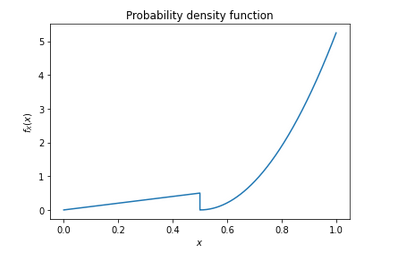
\includegraphics[width=\columnwidth]{solutions/ec/52/figures/pdfimage.png}
\caption{Graph of $f_X(x)$}
\end{figure}
\begin{equation} \label{ec52:eq9}
    F_X(x) = f_X(X<=x) = \int\limits_{-\infty}^x f_X(x) \, dx
\end{equation}
from $f_X(x)$ and equation \eqref{ec52:eq9}, 
\begin{displaymath}
    F_X(x)=\lcbrak{
                    \begin{array}{ll}
                        0 & x\leq 0 \\\\
		                \frac{x^2}{2} &   0 \leq x \leq \frac{1}{2}  \\\\
		                \frac{1}{8} + \frac{7}{8} (2x-1)^3 & \frac{1}{2} \leq x \leq 1 \\\\
		                1 & x>1\\
	                \end{array}    
                }
\end{displaymath}
\begin{figure}[!ht]
\centering
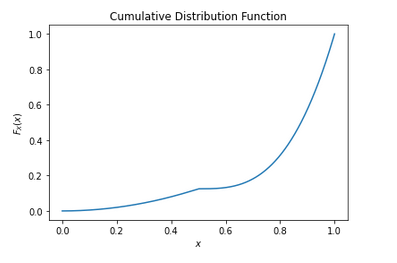
\includegraphics[width=\columnwidth]{solutions/ec/52/figures/cdfimage.png}
\caption{Graph of $F_X(x)$}
\end{figure}

